\section{Analyse af vognens overførelsesfunktion}\label{sec:sec_motoroverforelse}
\begin{wrapfigure}{r}{0.5\textwidth}
	\centering
	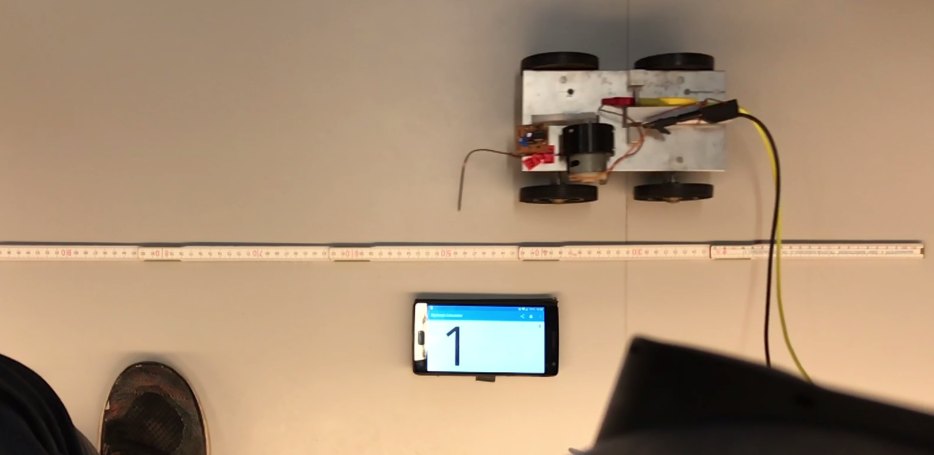
\includegraphics[width=.48\textwidth]{billeder/testopstilling_vogn.png}
	\caption{Testopstilling for accelerations måling af vogn.}
	\label{fig:testopstilling_vogn}
\end{wrapfigure}
\FloatBlock

Da systemet bliver bygget på en eksisterende vogn, hvis dynamik ikke er kendt, må der derfor findes en måde at modellere denne.
I forgående afsnit om pendulets dynamik fremkom det, at en acceleration af vognen kan påvirke en ændring af pendulet.
Generelt for en DC-motor gælder, at den påførte spænding har relation til rotationshastigheden af motoren og strømmen til motorens acceleration.    
For motoren er det kun kendt at den kommer fra Johnson Electric\footnote{\url{http://www.johnsonelectric.com/en/product-technology/motion/dc-motors}} og at den virker ved max. $12 \si{\volt}$\footnote{Motoren kan muligvis klare en højere spænding, men blev kun testet op til $12\si{\volt}$}. 

Under acceleration, vil DC-motoren trække den nødvendige strøm for at opnå den, af spændingens, fastsatte hastighed. 
Det antages at vognens acceleration er konstant for en given strøm så derfor vælges en testopstilling (se figur \ref{fig:testopstilling_vogn}), hvor der med konstant spænding til motoren måles på vognens acceleration ved faste strømbegrænsninger.
For alle målinger gælder, at vognen står stille ved start.
Herefter tændes for de strømbegrænsede strømforsyninger der er direkte tilsluttet DC-motoren. 

Der anvendes en konstant spænding til alle tests på $6 \si{\volt}$\footnote{Spændingen på  $6 \si{\volt}$ er valgt ud fra kravet om batteridrift, og den minimale spænding disse kan levere.}.
Acceleration optages på video med 240 fps. over en strækning af ca. $1 \si{\meter}$ hvorefter opmålingen foretages ved videoanalyse i Tracker\footnote{Tracker, Open Source Physics (OSP) - Video Analysis and Modeling Tool \url{http://physlets.org/tracker/}}.
I tabel \ref{tab:maaldata_vogn} er de valgte strømbegrænsninger angivet.

\begin{figure}
	\centering
	\subbottom[]{%
		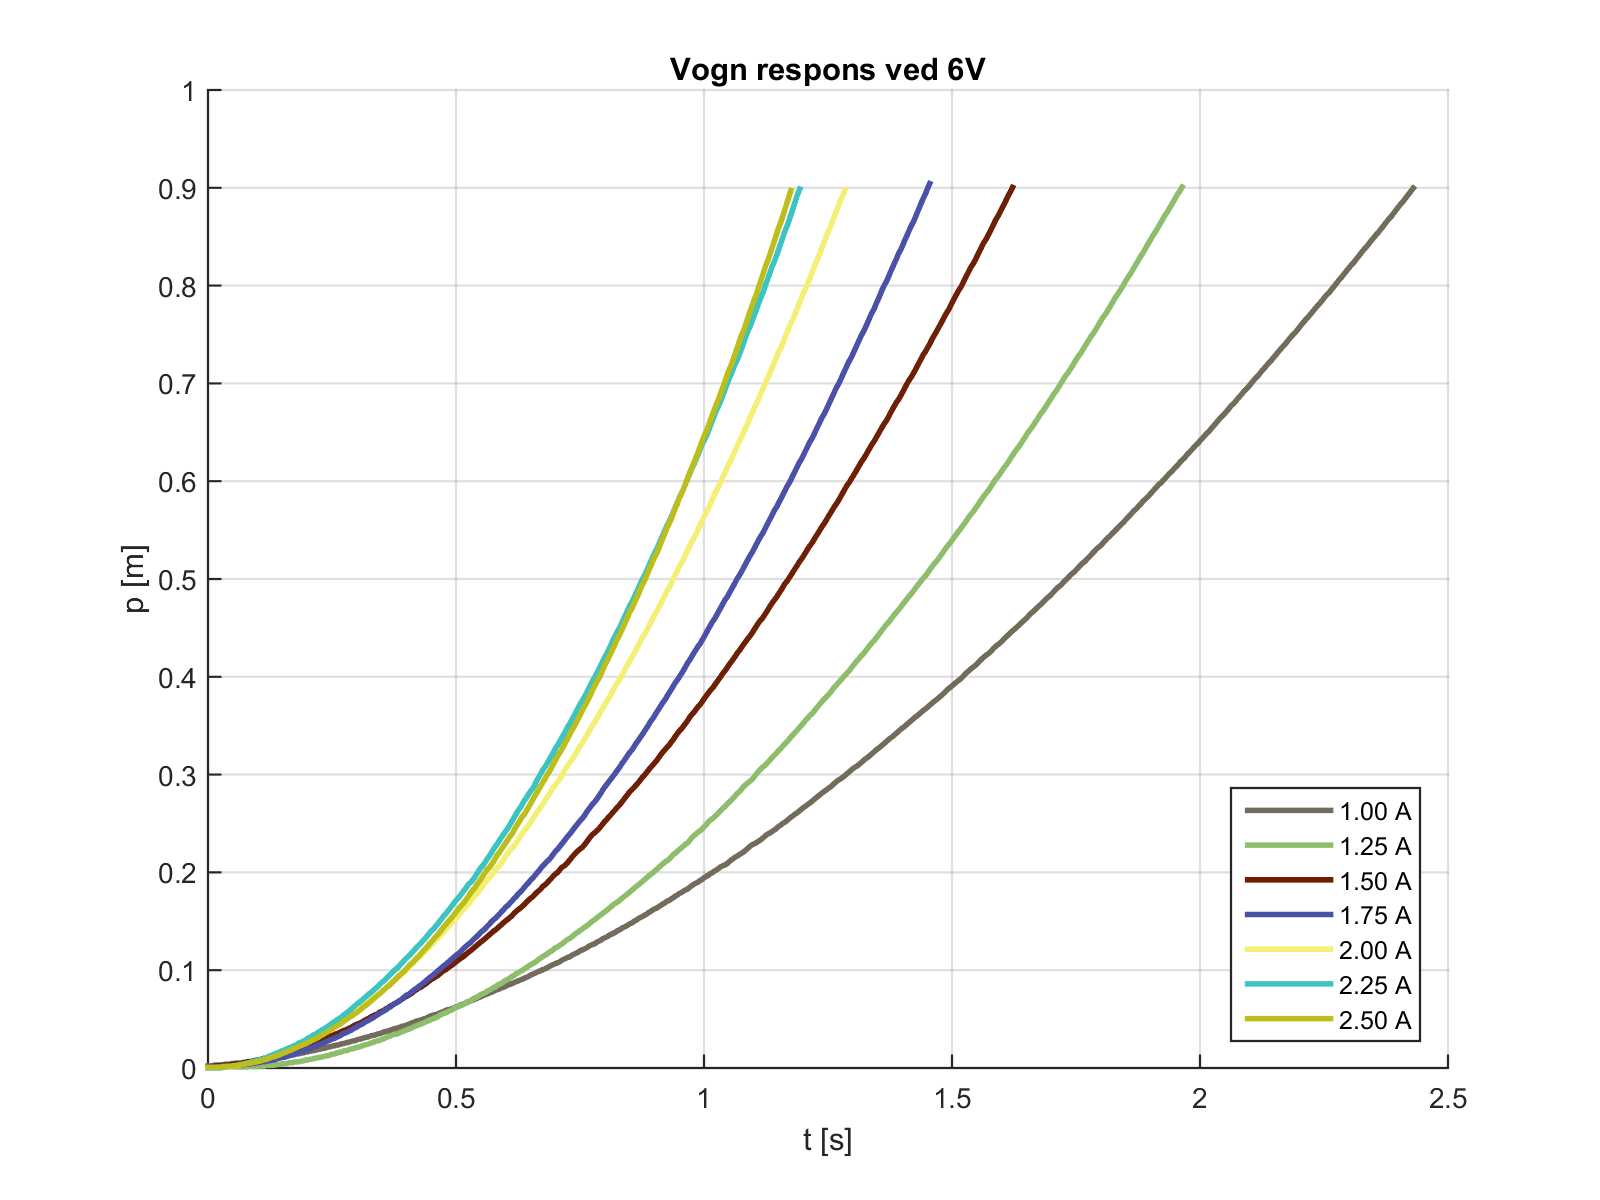
\includegraphics[width=.49\textwidth]{billeder/vogn_response_a.png}
		\label{fig:vogn_response_a}}
	\subbottom[]{%
		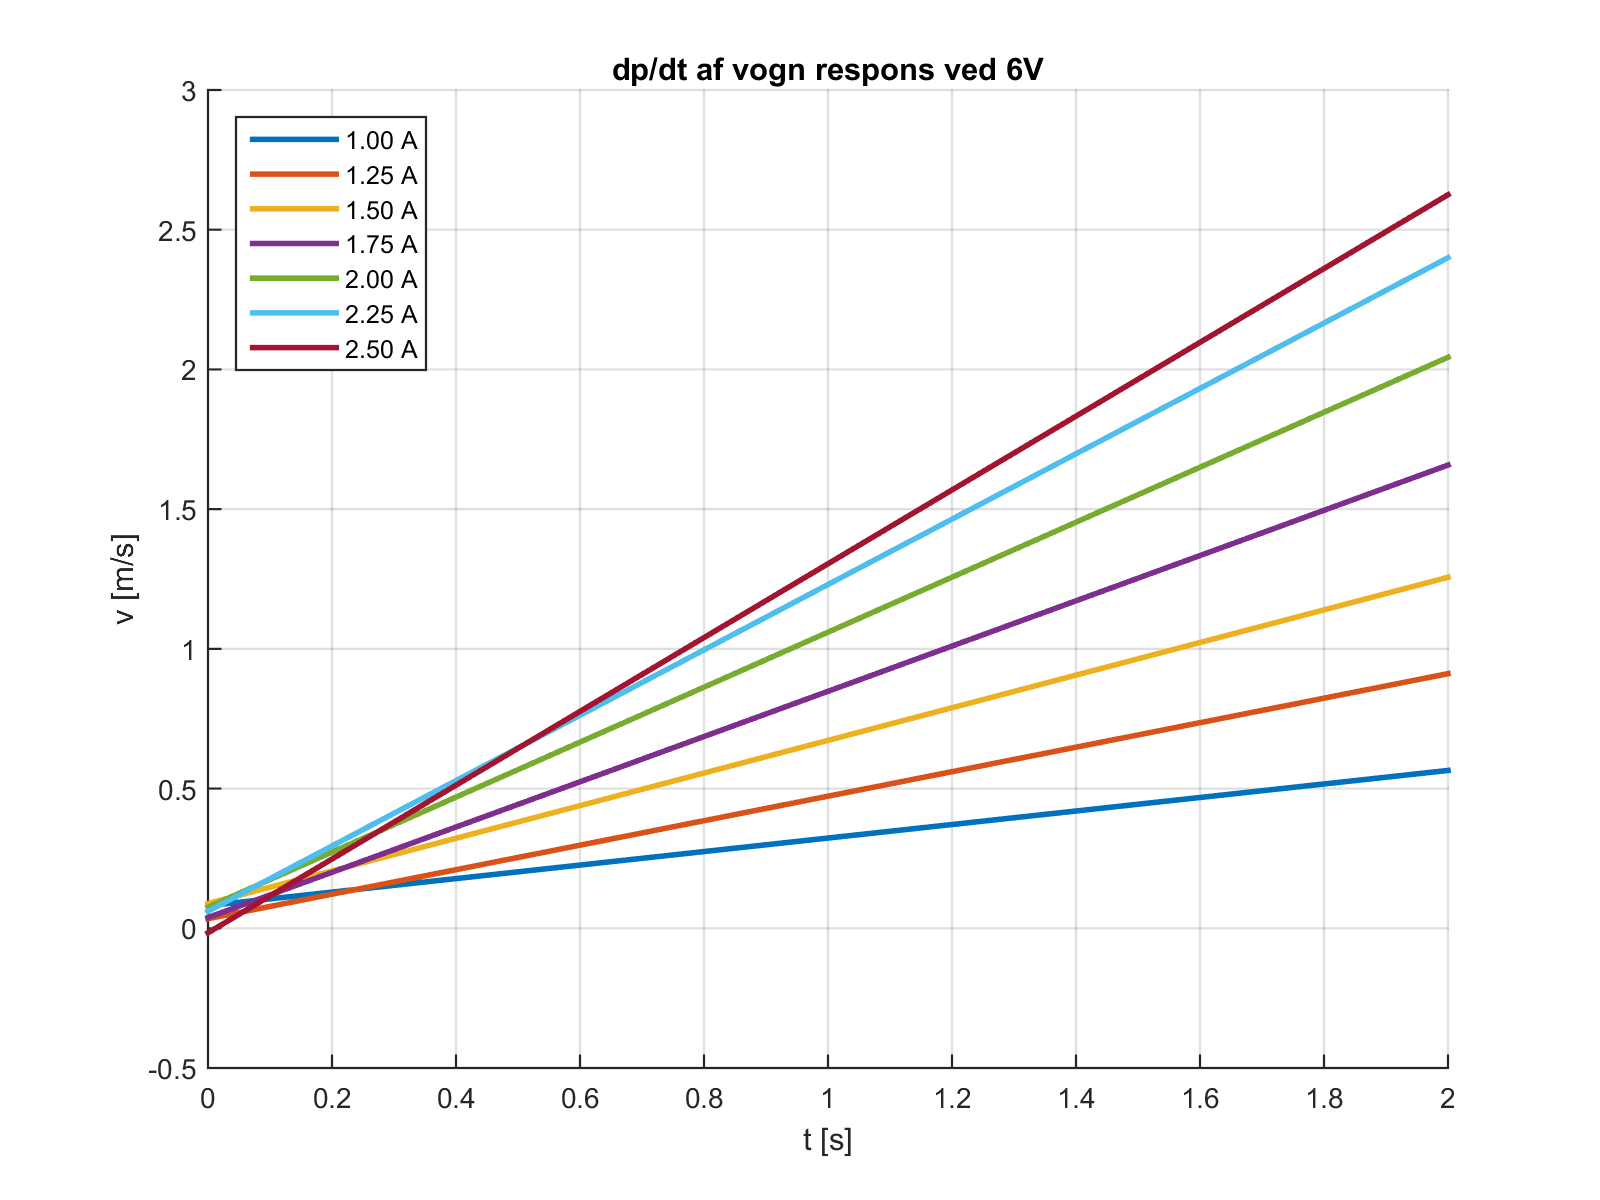
\includegraphics[width=.49\textwidth]{billeder/vogn_response_fit.png}
		\label{fig:vogn_responsefit}}
	\caption[Vognens position $p(t)$ og hasighed $v(t)$]{Vognens position $p$ som funktion af tiden $t$ ved strømbegrænsninger angivet i tabel \ref{tab:maaldata_vogn} (a) og $dp/dt$ af samme (b).}
	\label{fig:vogn_respose_mes}
\end{figure}

Efter databehandling afsættes alle målinger i en graf som ses i figur \ref{fig:vogn_response_a}.
Grafen viser vognens position som funktion af tiden $p(t)|_{I=n}$.
Ved hjælp af MATLAB beregnes nu vognens hastighed og acceleration ved 
\begin{align}
v = \frac{d}{dt}p(t) \quad\quad a= \frac{d^2}{dt^2}p(t)
\end{align}
I figur \ref{fig:vogn_responsefit} er vognens hastighed afsat som funktion af tiden.
Her ses, at for hver strømbegrænsning, har vognen en konstant acceleration $dv(t)/dt$
De fundne accelerationer og tilhørende strømbegrænsninger er afsat i figur \ref{fig:vogn_response}.


\begin{figure}[h!]
	\centering
	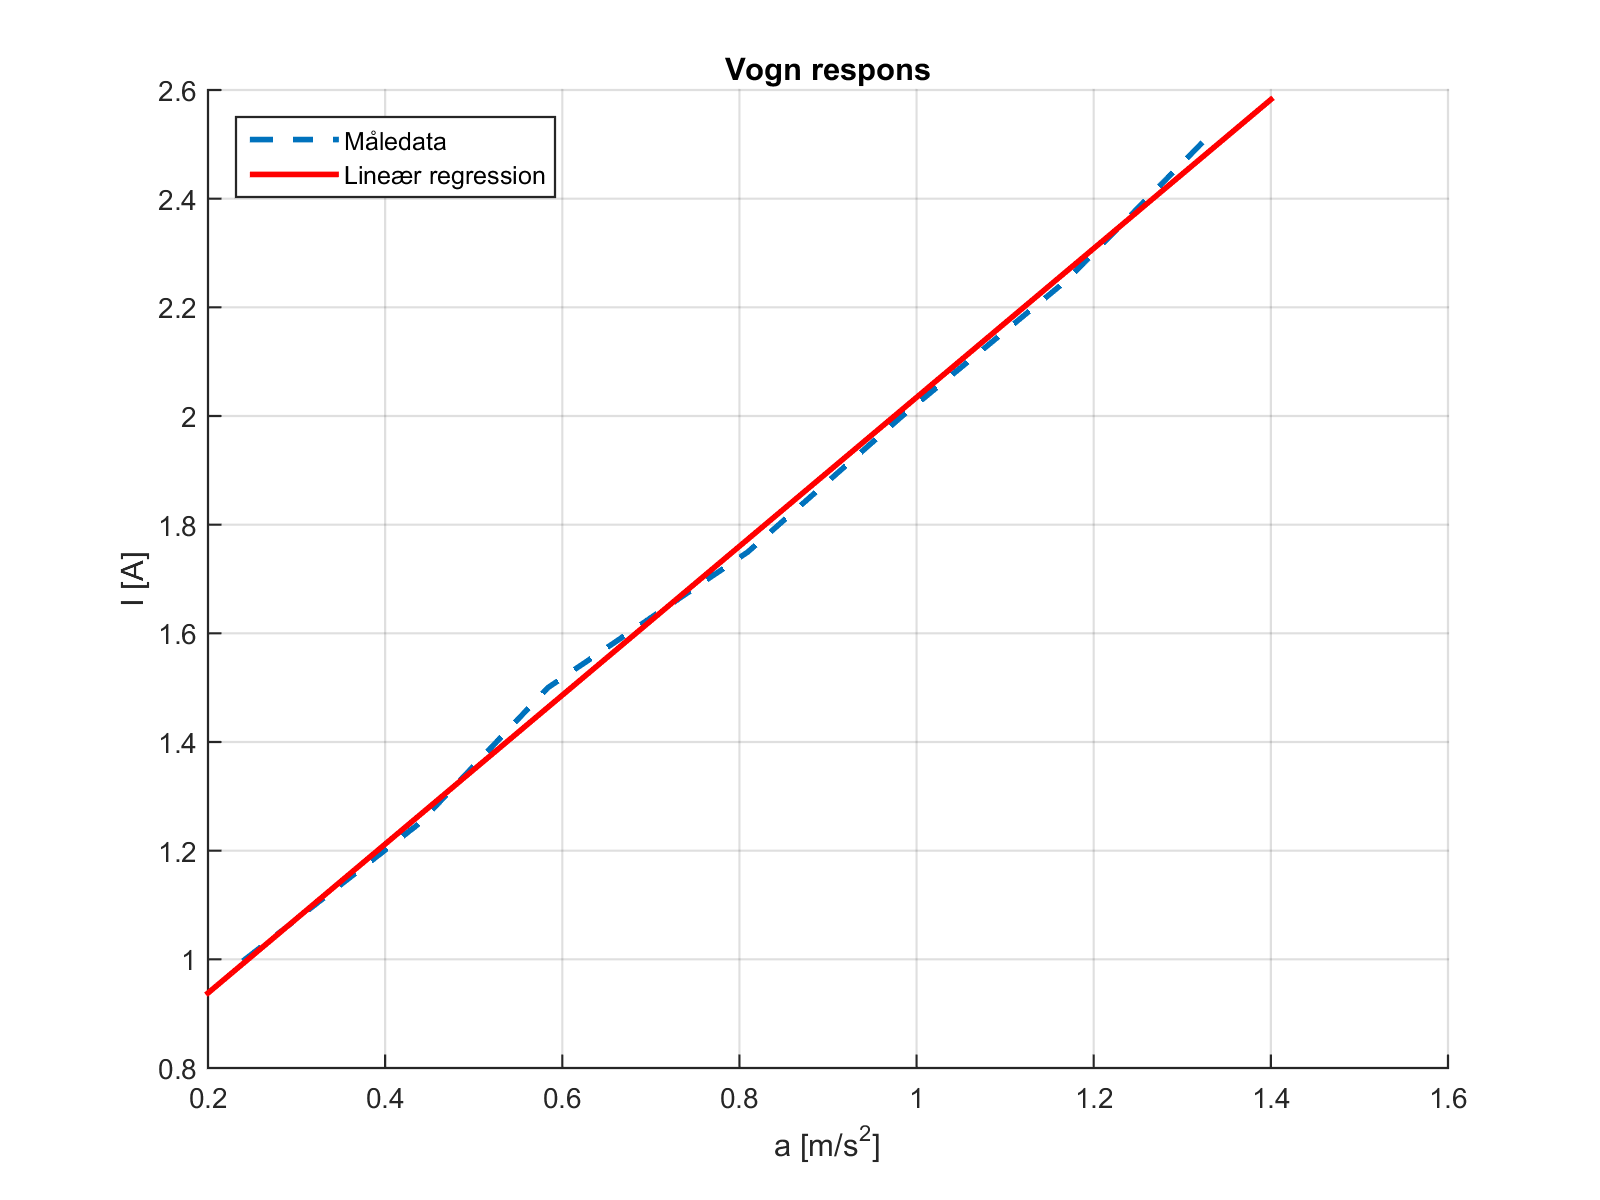
\includegraphics[width=.8\textwidth]{billeder/vogn_response.png}
	\caption[Vognens respons $I(a)$]{Vognens respons beskrevet som $I(a)$. Den stiplede blå linje viser måledata. Den røde viser resultatet af lineær regression.}
	\label{fig:vogn_response}
\end{figure}

Ved lineær regression på resultaterne af målinger i tabel \ref{tab:maaldata_vogn}, som er afbilledet i figur \ref{fig:vogn_response} fås en hældningskoefficient på $k_v = 1,3704$ 
Således viser antagelsen om konstant acceleration i det arbejdsområde vi ønsker at holde stik.
Vognens dynamik kan således beskrives som
\begin{align}
I(a) = 1,37a + 0,6639  \label{eq:vogn_dynamic}
\end{align} 
Den Laplace-transformerede af ligning \ref{eq:vogn_dynamic} er således
\begin{align}
\lapl{ \left[ I(a) \right]} = I(s) = \frac{0,66s + 1,37}{s^2} = \frac{0,66}{s} + \frac{1,37}{s^2} \label{eq:vogn_dynamic_trans}
\end{align}

\begin{table}[h!]
	\small
	\centering
	\caption{Måledata for vognens acceleration.}
	\label{tab:maaldata_vogn}
	\begin{threeparttable}
		\begin{tabular}{ l l l l l l l }
			\toprule
			\multicolumn{1}{l}{\textbf{Test}}       &
			\multicolumn{1}{l}{\textbf{Strøm begrænsning [\si{\ampere}]}}       &
			\multicolumn{1}{l}{\textbf{Acceleration [\si{\meter\per\second\squared}]}}   \\ 
			\hline
			1 &  1,00  &  \num{0.2419}  \\
			2 &  1,25  &  \num{0.4384}  \\
			3 &  1,50  &  \num{0.5838}  \\
			4 &  1,75  &  \num{0.8096}  \\
			5 &  2,00  &  \num{0.9838}  \\
			6 &  2,25  &  \num{1.1696}  \\
			7 &  2,50  &  \num{1.3207}  \\
			\hline
			\bottomrule
		\end{tabular}
		%\begin{tablenotes}
		%\item[a] \textit{Maximum værdi fra datablad}
		%\end{tablenotes}
	\end{threeparttable}
\end{table} 

\section{Delkonklusion for vognens dynamik}

I ligning \ref{eq:vogn_dynamic_trans} er der således fremkommet en beskrivelse af vognens dynamik, som senere kan anvendes til at beskrive hele systemet og dimensionering af regulatoren.
Denne og bestemmelsen af overførelses funktionen for det fysiske system af pendul og vogn, giver to vigtige byggeklodser til at bestemme overførelses funktionen for hele systemet, som udledes i kapitel \ref{chap:motor_reg}.
Under test af vognens acceleration gav en for høj strøm ($I > 2,25 \si{\ampere} $ ), anledning til hjulspin og en for lav strøm ($I < 1,00 \si{\ampere} $ ) var ikke i stand til at sætte vognen i bevægelse.
Derfor vælges et område på ($ 1,00 \si{\ampere} <  I < 2,25 \si{\ampere} $ ) som det arbejdsområde vi ønsker at styre med motorstyringen, der bliver beskrevet i kapitel \ref{chap:motor_reg}
\husk{JJ}{Lidt mere diskussion og konklusion til dette kapitel}



 